\chapter{Detailed overview of all solutions}\label{chapter:allsolutions}

\def \nameofversion {Design}
\subsection*{The design lattice}
\pdfbookmark[section]{The design lattice}{The design lattice}
\begin{figure}[htbp!]
	\centering
	\includegraphics[width = \textwidth]{images/04-design-lattice.pdf}
	\caption{The design lattice of the Bessy II storage ring (1996).}
\end{figure}
\begin{table}[htbp!]
	\centering
	\footnotesize
	\caption{Quadrupole strengths of the design lattice.}
	\begin{tabular}{rrrrrr}
	\toprule
 $Q_{\textup{x}}$ / kHz &  $Q_{\textup{y}}$ / kHz &  $\beta_{\textup{x,max}}$ / m &  $\beta_{\textup{y,max}}$ / m &  $\overline{\beta}_{\textup{x,rel}}$ / m &  $\overline{\beta}_{\textup{y,rel}}$ / m \\
	\midrule
1061.71  &                  928.03 &                        17.6 &                         21.09    &                                      1.18  &                                    1.02 \\
\bottomrule
\end{tabular}
\\\begin{tabular}{lr}
\toprule
\textbf{Magnet} & \textbf{k} / m$^{-2}$\\
\midrule
Q1	& +2.45190 \\
Q2	& -1.89757\\
Q3D	& -2.02025\\
Q4D & +1.40816\\
Q3T & -2.46319\\
Q4T & +2.62081\\
Q5T & -2.60000\\
\bottomrule \\ \\
\end{tabular}


\end{table}
\newpage


\def \nameofversion {current}
\subsection*{The current standard lattice}
\pdfbookmark[section]{The current standard lattice}{The current standard lattice}
\begin{figure}[htbp!]
	\centering
	\includegraphics[width = \textwidth]{images/Overview-all-solutions/\nameofversion-comparison.pdf}
	\caption{The current standard lattice of the Bessy II storage ring (28.03.2017).}
\end{figure}
\begin{table}[htbp!]
	\centering
	\footnotesize
	\caption{Quadrupole strengths of the current standard lattice.}
	\begin{tabular}{rrrrrr}
	\toprule
 $Q_{\textup{x}}$ / kHz &  $Q_{\textup{y}}$ / kHz &  $\beta_{\textup{x,max}}$ / m &  $\beta_{\textup{y,max}}$ / m &  $\overline{\beta}_{\textup{x,rel}}$ / m &  $\overline{\beta}_{\textup{y,rel}}$ / m \\
	\midrule
 1060.54 &                  907.38 &                         26.14 &                         24.00 &                                     1.00 &                                     1.00 \\
\end{tabular}
\\\begin{tabular}{ll}
\toprule
\textbf{Magnet} & \textbf{k} / m$^{-2}$\\
\midrule
QIT6       & -1.09324443\\
Q1D        & +2.43992187\\
Q2D        & -1.85354137\\
Q3P1T1     & -2.53759435\\
Q3P1T6     & -2.68493846\\
Q3P1T8     & -2.44627319\\
Q3P2T1     & -2.44026692\\
Q3P2T6     & -2.33722602\\
Q3P2T8     & -2.53960920\\
Q3D1       & -2.02056340\\
Q3D2       & -2.12545914\\
Q3D3       & -2.12560233\\
Q3D4       & -2.13235047\\
Q3D5       & -2.11955588\\
Q3D6       & -2.10963250\\
Q3D7       & -2.11735207\\
Q3D8       & -2.13655479\\
\bottomrule \\ \\
\end{tabular}
\begin{tabular}{ll}
\toprule
\textbf{Magnet} & \textbf{k} / m$^{-2}$\\
\midrule
Q3T2       & -2.45516822\\
Q3T3       & -2.42796219\\
Q3T4       & -2.43958732\\
Q3T5       & -2.44973680\\
Q3T7       & -2.43215097\\
Q4P1T1     & +2.61530699\\
Q4P1T6     & +2.24854535\\
Q4P1T8     & +2.58252211\\
Q4P2T1     & +2.58203605\\
Q4P2T6     & +2.56031750\\
Q4P2T8     & +2.62213165\\
Q4D1       & +1.40197290\\
Q4D2       & +1.47885355\\
Q4D3       & +1.48649031\\
Q4D4       & +1.49263679\\
Q4D5       & +1.47760503\\
Q4D6       & +1.48292220\\
Q4D7       & +1.47659449\\
Q4D8       & +1.49275949\\
\bottomrule
\end{tabular}
\begin{tabular}{ll}
\toprule
\textbf{Magnet} & \textbf{k} / m$^{-2}$\\
\midrule
Q4T2       & +2.57898949\\
Q4T3       & +2.57796719\\
Q4T4       & +2.58157782\\
Q4T5       & +2.58022594\\
Q4T7       & +2.58000776\\
Q5P1T1     & -2.42116424\\
Q5P1T6     & -1.02671552\\
Q5P1T8     & -2.59460394\\
Q5P2T1     & -2.60077137\\
Q5P2T6     & -2.45473858\\
Q5P2T8     & -2.41402770\\
Q5T2       & -2.58798946\\
Q5T3       & -2.62810235\\
Q5T4       & -2.59997779\\
Q5T5       & -2.59005859\\
Q5T7       & -2.60805533\\
\bottomrule \\ \\ \\
\end{tabular}

	\label{tab:standard2017quadsrengths}
\end{table}
\newpage


\def \nameofversion {V1}
\subsection*{\nameofversion}
\pdfbookmark[section]{\nameofversion}{\nameofversion}
\begin{figure}[htbp!]
	\centering
	\includegraphics[width = \textwidth]{images/Overview-all-solutions/\nameofversion-comparison.pdf}
	\caption{Comparison of the \nameofversion -lattice with the current lattice.}
\end{figure}
\begin{table}[htbp!]
	\centering
	\footnotesize
	\caption{Fit output \nameofversion.}
	\input{tables/\nameofversion.tex}
\end{table}
\newpage

\def \nameofversion {V2}
\subsection*{\nameofversion}
\pdfbookmark[section]{\nameofversion}{\nameofversion}
\begin{figure}[htbp!]
	\centering
	\includegraphics[width = \textwidth]{images/Overview-all-solutions/\nameofversion-comparison.pdf}
	\caption{Comparison of the \nameofversion -lattice with the current lattice.}
\end{figure}
\begin{table}[htbp!]
	\centering
	\footnotesize
	\caption{Fit output \nameofversion.}
	\input{tables/\nameofversion.tex}
\end{table}
\newpage

\def \nameofversion {V3}
\subsection*{\nameofversion}
\pdfbookmark[section]{\nameofversion}{\nameofversion}
\begin{figure}[htbp!]
	\centering
	\includegraphics[width = \textwidth]{images/Overview-all-solutions/\nameofversion-comparison.pdf}
	\caption{Comparison of the \nameofversion -lattice with the current lattice.}
\end{figure}
\begin{table}[htbp!]
	\centering
	\footnotesize
	\caption{Fit output \nameofversion.}
	\input{tables/\nameofversion.tex}
\end{table}
\newpage



\def \nameofversion {V4}
\subsection*{\nameofversion}
\pdfbookmark[section]{\nameofversion}{\nameofversion}
\begin{figure}[htbp!]
	\centering
	\includegraphics[width = \textwidth]{images/Overview-all-solutions/\nameofversion-comparison.pdf}
	\caption{Comparison of the \nameofversion -lattice with the current lattice.}
\end{figure}
\begin{table}[htbp!]
	\centering
	\footnotesize
	\caption{Fit output \nameofversion.}
	\input{tables/\nameofversion.tex}
\end{table}
\newpage




\def \nameofversion {V5}
\subsection*{\nameofversion}
\pdfbookmark[section]{\nameofversion}{\nameofversion}
\begin{figure}[htbp!]
	\centering
	\includegraphics[width = \textwidth]{images/Overview-all-solutions/\nameofversion-comparison.pdf}
	\caption{Comparison of the \nameofversion -lattice with the current lattice.}
\end{figure}
\begin{table}[htbp!]
	\centering
	\footnotesize
	\caption{Fit output \nameofversion.}
	\input{tables/\nameofversion.tex}
\end{table}
\newpage



\def \nameofversion {Vall}
\subsection*{\nameofversion}
\pdfbookmark[section]{\nameofversion}{\nameofversion}
\begin{figure}[htbp!]
	\centering
	\includegraphics[width = \textwidth]{images/Overview-all-solutions/\nameofversion-comparison.pdf}
	\caption{Comparison of the \nameofversion -lattice with the current lattice.}
\end{figure}
\begin{table}[htbp!]
	\centering
	\footnotesize
	\caption{Fit output \nameofversion.}
	\input{tables/\nameofversion.tex}
\end{table}
\newpage



\def \nameofversion {V2Q3T}
\subsection*{\nameofversion}
\pdfbookmark[section]{\nameofversion}{\nameofversion}
\begin{figure}[htbp!]
	\centering
	\includegraphics[width = \textwidth]{images/Overview-all-solutions/\nameofversion-comparison.pdf}
	\caption{Comparison of the \nameofversion -lattice with the current lattice.}
\end{figure}
\begin{table}[htbp!]
	\centering
	\footnotesize
	\caption{Fit output \nameofversion.}
	\input{tables/\nameofversion.tex}
\end{table}
\newpage


\def \nameofversion {V2Q4T}
\subsection*{\nameofversion}
\pdfbookmark[section]{\nameofversion}{\nameofversion}
\begin{figure}[htbp!]
	\centering
	\includegraphics[width = \textwidth]{images/Overview-all-solutions/\nameofversion-comparison.pdf}
	\caption{Comparison of the \nameofversion -lattice with the current lattice.}
\end{figure}
\begin{table}[htbp!]
	\centering
	\footnotesize
	\caption{Fit output \nameofversion.}
	\input{tables/\nameofversion.tex}
\end{table}
\newpage


\def \nameofversion {V2Q5}
\subsection*{\nameofversion}
\pdfbookmark[section]{\nameofversion}{\nameofversion}
\begin{figure}[htbp!]
	\centering
	\includegraphics[width = \textwidth]{images/Overview-all-solutions/\nameofversion-comparison.pdf}
	\caption{Comparison of the \nameofversion -lattice with the current lattice.}
\end{figure}
\begin{table}[htbp!]
	\centering
	\footnotesize
	\caption{Fit output \nameofversion.}
	\input{tables/\nameofversion.tex}
\end{table}
\newpage

\def \nameofversion {VOF}
\subsection*{\nameofversion}
\pdfbookmark[section]{\nameofversion}{\nameofversion}
\begin{figure}[htbp!]
	\centering
	\includegraphics[width = \textwidth]{images/Overview-all-solutions/\nameofversion-comparison.pdf}
	\caption{Comparison of the \nameofversion -lattice with the current lattice.}
\end{figure}
\begin{table}[htbp!]
	\centering
	\footnotesize
	\caption{Fit output \nameofversion.}
	\input{tables/\nameofversion.tex}
\end{table}
\newpage


\subsection*{LOCO measurements}
\pdfbookmark[section]{LOCO measurements of the new optics}{LOCO measurements of the new optics}

\subsection*{V1: LOCO vs SIM}
\begin{figure}[htbp!]
	\centering
	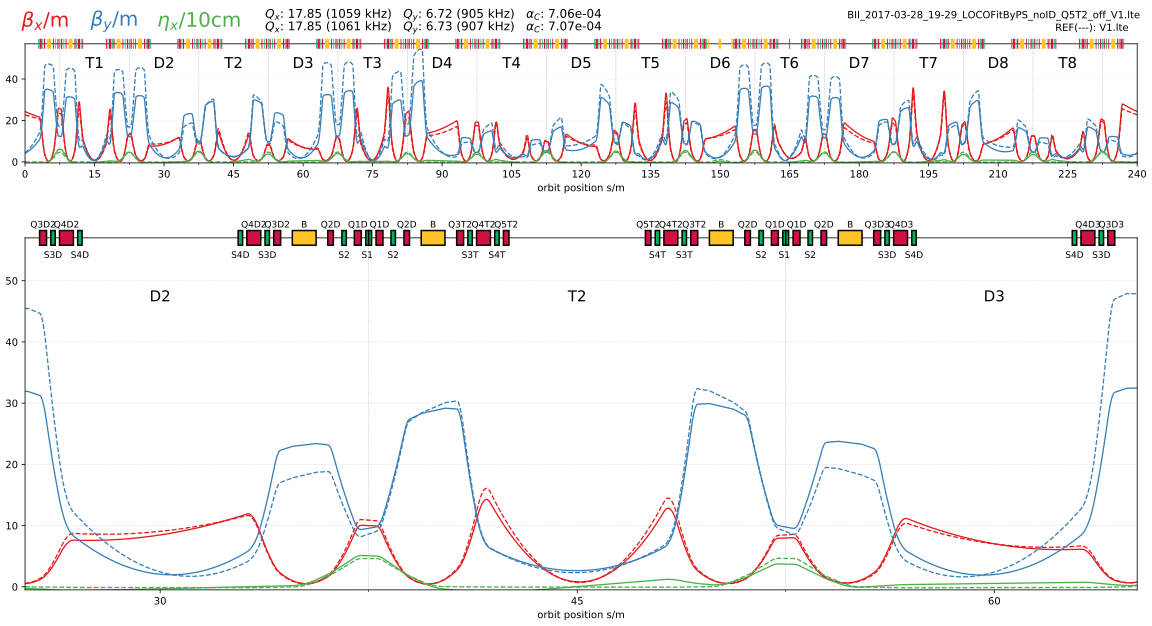
\includegraphics[width = \textwidth]{images/Overview-all-solutions/A-V1_LOCO_vs_SIM.pdf}
	\caption{Comparison of V1 LOCO (solid) with V1 SIM (dashed).}
	\label{fig:V1-LOCO-vs-SIM}
\end{figure}

\subsection*{V2: LOCO vs SIM}
\begin{figure}[htbp!]
	\centering
	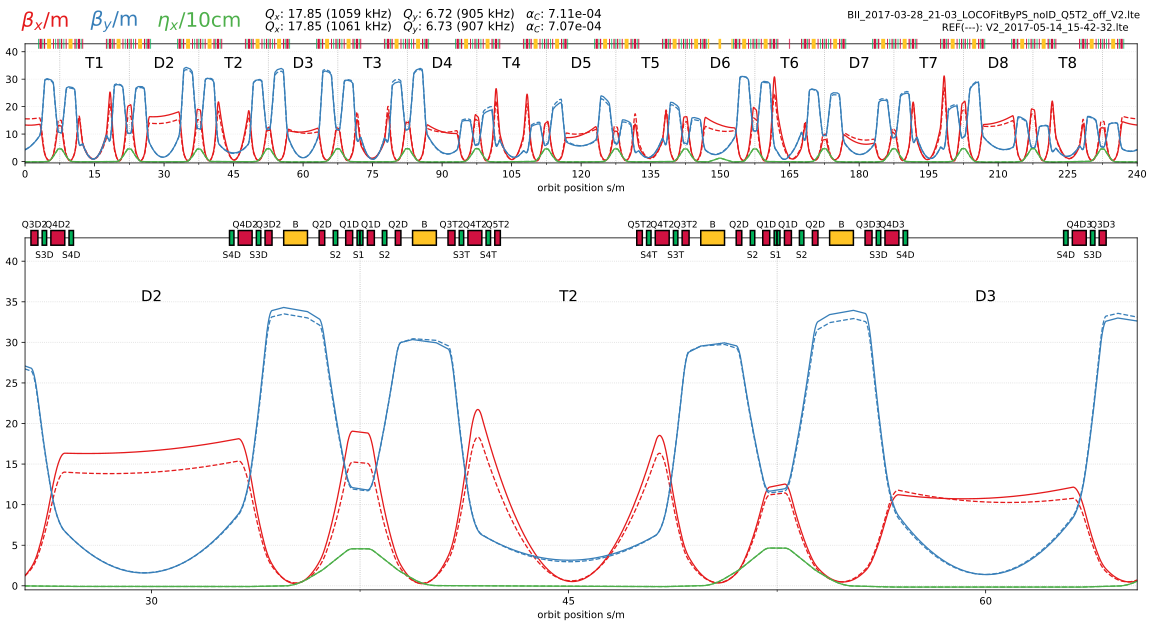
\includegraphics[width = \textwidth]{images/Overview-all-solutions/A-V2_LOCO_vs_SIM.pdf}
	\caption{Comparison of V2 LOCO (solid) with V2 SIM (dashed).}
	\label{fig:V2-LOCO-vs-SIM}
\end{figure}


\newpage
\subsection*{V4 LOCO vs SIM (MAY)}
\begin{figure}[htbp!]
	\centering
	\includegraphics[width = \textwidth]{images/05-V4_LOCO_vs_SIM.pdf}
	\caption{Comparison of V4 LOCO (solid) with V4 SIM (dashed) of May.}
\end{figure}

\subsection*{V4 LOCO vs SIM LOCO (AUG)}
\begin{figure}[htbp!]
	\centering
	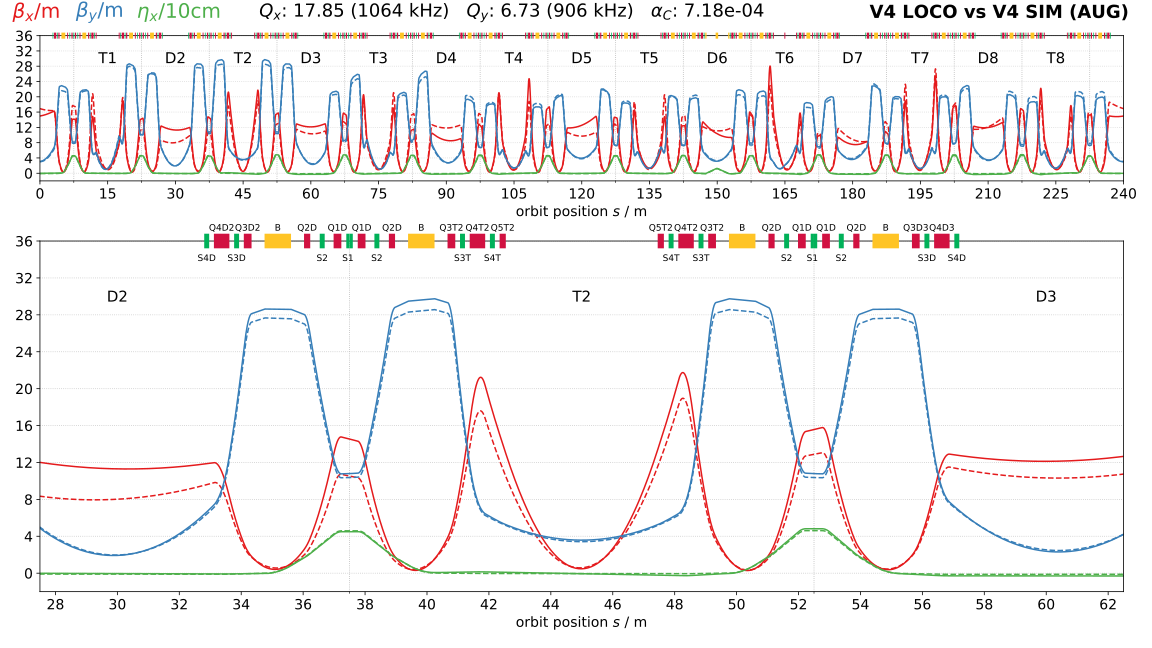
\includegraphics[width = \textwidth]{images/Overview-all-solutions/A-V4_LOCO_vs_SIM_AUG.pdf}
	\caption{Comparison of V4 LOCO (solid) with V4 SIM (dashed) of August.}
	\label{fig:V4-LOCO-vs-SIM_AUG}
\end{figure}


\newpage
\subsection*{V4 LOCO August vs Stanard LOCO}
\begin{figure}[htbp!]
	\centering
	\includegraphics[width = \textwidth]{images/05-V4_vs_standard_loco.pdf}
	\caption{The loco measured V4 optics (solid) in comparison to the standard optics (dashed).}
\end{figure}


\subsection*{Standard: August vs March}
\begin{figure}[htbp!]
	\centering
	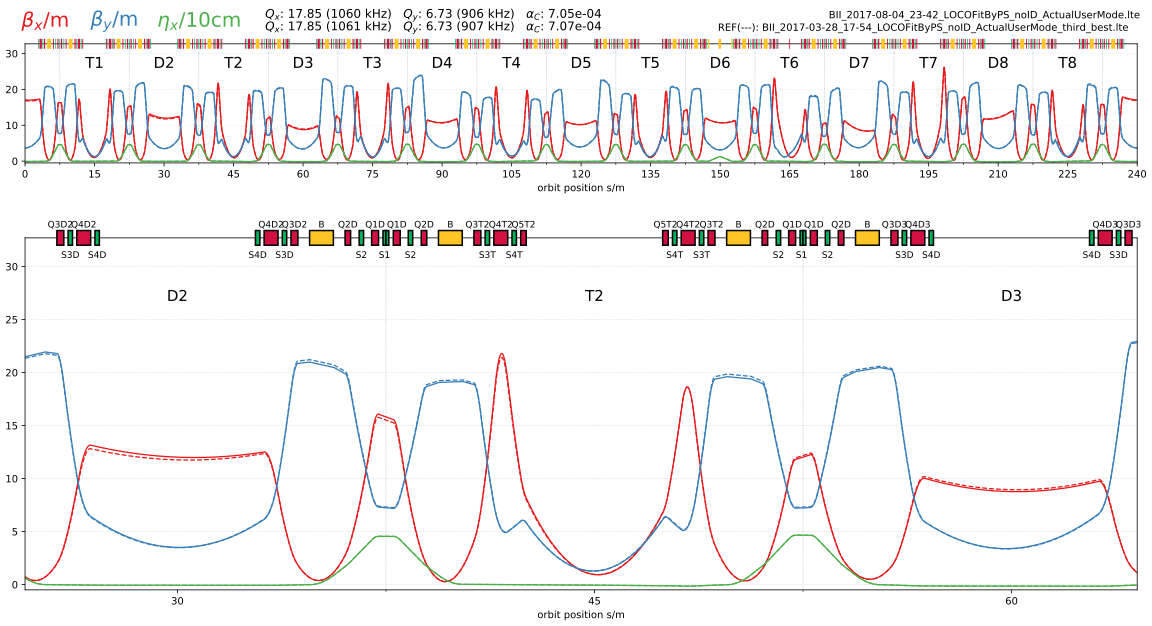
\includegraphics[width = \textwidth]{images/Overview-all-solutions/A-comparison-standard-optics-august-vs-march.pdf}
	\caption{Comparison of the LOCO measured standard optics from 04.08.2017 with 28.03.2017.}
	\label{fig:standard-comparison}
\end{figure}



